\begin{table}[!h]
\centering
\caption{Monte Carlo Design Parameters}
\label{tab:mc_design}
\begin{tabular}{ccccc}
\toprule
Sample Size $n$ & Subsample Size $b$ & Non-overlapping Blocks $N_b$ & MC Replications $M$ \\
\midrule
500 & 62 & 8 & 200 \\
1{,}000 & 99 & 10 & 200 \\
10{,}000 & 464 & 21 & 200 \\
100{,}000 & 2{,}154 & 46 & 200 \\
500{,}000 & 6{,}299 & 79 & 200 \\
\bottomrule
\end{tabular}
\begin{flushleft}
\footnotesize\textit{Notes:} The subsample size is set to $b = \lfloor n^{2/3} \rfloor$ following \cite{PR99}.  $N_b = \lfloor n/b \rfloor$ denotes the number of non-overlapping blocks per replication.
\end{flushleft}
\end{table}


\begin{table}[!h]
\centering
\caption{Summary of unrestricted subsampling results (reparameterized space)}
\label{tab:subsampling_summary}
\resizebox{\textwidth}{!}{%
\begin{tabular}{lccccccccccc}
\toprule
& & & & & & & \multicolumn{2}{c}{Quantile CI} & \multicolumn{2}{c}{Normal CI} \\
\cmidrule(lr){8-9} \cmidrule(lr){10-11}
$n$ & Param.\ & True & Avg.\ Est.\ & Std.\ Est.\ & Dev.\ Mean & Skew & Kurt & qCov90 & qCov95 & nCov90 & nCov95 \\
\midrule
\multirow{5}{*}{$500$}
& $\psi_1$ & 0.80 & 0.810 & 0.098 & $-0.14$ & $-0.59$ & $0.36$ & 0.495 & 0.525 & 0.650 & 0.720 \\
& $\psi_2$ & 0.30 & 0.282 & 0.207 & $0.69$ & $0.15$ & $-0.28$ & 0.350 & 0.350 & 0.475 & 0.535 \\
& $\sigma$ & 1.60 & 1.537 & 0.218 & $-0.06$ & $0.32$ & $-0.07$ & 0.565 & 0.590 & 0.615 & 0.730 \\
& $\pi_1$ & 0.4375 & 0.394 & 0.181 & $-0.45$ & $0.28$ & $-0.26$ & 0.360 & 0.405 & 0.515 & 0.590 \\
& $\alpha$ & 1.50 & 1.501 & 0.121 & $0.41$ & $-0.09$ & $-0.58$ & 0.655 & 0.680 & 0.780 & 0.840 \\
\midrule
\multirow{5}{*}{$1{,}000$}
& $\psi_1$ & 0.80 & 0.803 & 0.073 & $-0.05$ & $-0.32$ & $0.00$ & 0.605 & 0.650 & 0.785 & 0.810 \\
& $\psi_2$ & 0.30 & 0.269 & 0.161 & $0.92$ & $0.15$ & $-0.51$ & 0.455 & 0.460 & 0.620 & 0.690 \\
& $\sigma$ & 1.60 & 1.566 & 0.157 & $-0.34$ & $0.27$ & $-0.08$ & 0.685 & 0.720 & 0.760 & 0.815 \\
& $\pi_1$ & 0.4375 & 0.429 & 0.144 & $-0.87$ & $0.24$ & $-0.10$ & 0.380 & 0.450 & 0.565 & 0.655 \\
& $\alpha$ & 1.50 & 1.502 & 0.079 & $0.34$ & $-0.11$ & $-0.51$ & 0.790 & 0.835 & 0.865 & 0.920 \\
\midrule
\multirow{5}{*}{$10{,}000$}
& $\psi_1$ & 0.80 & 0.801 & 0.019 & $0.21$ & $0.22$ & $-0.50$ & 0.865 & 0.900 & 0.920 & 0.970 \\
& $\psi_2$ & 0.30 & 0.293 & 0.044 & $0.23$ & $0.13$ & $-0.77$ & 0.780 & 0.795 & 0.890 & 0.945 \\
& $\sigma$ & 1.60 & 1.597 & 0.051 & $-1.25$ & $0.11$ & $-0.44$ & 0.830 & 0.865 & 0.845 & 0.920 \\
& $\pi_1$ & 0.4375 & 0.437 & 0.039 & $-1.05$ & $-0.31$ & $-0.41$ & 0.830 & 0.855 & 0.905 & 0.945 \\
& $\alpha$ & 1.50 & 1.501 & 0.026 & $0.15$ & $-0.08$ & $-0.10$ & 0.895 & 0.955 & 0.900 & 0.940 \\
\midrule
\multirow{5}{*}{$100{,}000$}
& $\psi_1$ & 0.80 & 0.801 & 0.006 & $0.11$ & $0.94$ & $2.03$ & 0.940 & 0.970 & 0.935 & 0.990 \\
& $\psi_2$ & 0.30 & 0.301 & 0.013 & $-0.55$ & $-0.65$ & $0.64$ & 0.925 & 0.950 & 0.955 & 0.980 \\
& $\sigma$ & 1.60 & 1.599 & 0.015 & $-0.82$ & $-0.24$ & $0.19$ & 0.925 & 0.960 & 0.935 & 0.965 \\
& $\pi_1$ & 0.4375 & 0.436 & 0.012 & $-0.13$ & $-0.79$ & $1.96$ & 0.950 & 0.995 & 0.965 & 0.995 \\
& $\alpha$ & 1.50 & 1.501 & 0.008 & $0.07$ & $-0.01$ & $0.02$ & 0.905 & 0.940 & 0.890 & 0.950 \\
\midrule
\multirow{5}{*}{$500{,}000$}
& $\psi_1$ & 0.80 & 0.800 & 0.003 & $0.03$ & $0.49$ & $1.53$ & 0.925 & 0.965 & 0.910 & 0.950 \\
& $\psi_2$ & 0.30 & 0.299 & 0.006 & $-0.30$ & $-0.73$ & $1.63$ & 0.940 & 0.965 & 0.955 & 0.980 \\
& $\sigma$ & 1.60 & 1.599 & 0.006 & $-0.35$ & $-0.06$ & $0.14$ & 0.940 & 0.960 & 0.930 & 0.955 \\
& $\pi_1$ & 0.4375 & 0.437 & 0.005 & $0.01$ & $-0.33$ & $1.44$ & 0.925 & 0.970 & 0.930 & 0.965 \\
& $\alpha$ & 1.50 & 1.500 & 0.004 & $0.04$ & $0.01$ & $-0.01$ & 0.910 & 0.950 & 0.900 & 0.945 \\
\bottomrule
\end{tabular}%
}
\begin{flushleft}
\footnotesize\textit{Notes:} Avg.~Est.\ and Std.~Est.\ are the mean and standard deviation of $\hat{\vartheta}_n$ over $M=200$ replications.  Dev.~Mean, Skew, and Kurt are the mean, skewness and excess kurtosis of the non-overlapping block scaled deviations $Z^{(i)}_b$, pooled across replications.  qCov and nCov denote the average coverage of quantile-based and normal-approximation confidence intervals.  The full-sample and block estimators are the same functional, evaluated with identical starting values and optimizer tolerances.
\end{flushleft}
\end{table}


\begin{table}[htbp]
\centering
\caption{Subsampling results (reparameterized) for $n = 500$ ($b = 62$, $N_b = 8$, $M = 200$)}
\label{tab:subsampling_n500}
\resizebox{\textwidth}{!}{%
\begin{tabular}{lcccccccccccccc}
\toprule
& & & & & & & & & & \multicolumn{2}{c}{Quantile CI} & \multicolumn{2}{c}{Normal CI} \\
\cmidrule(lr){10-11} \cmidrule(lr){12-13}
Parameter & True & Avg Est.\ & Std Est.\ & Dev.\ Mean & Dev.\ Std & Skew & Kurt & SW Rej.\ & JB Rej.\ & qCov90 & qCov95 & nCov90 & nCov95 \\
\midrule
$\psi_1$ & 0.800 & 0.810 & 0.098 & $-0.14$ & 1.430 & $-0.59$ & $0.36$ & 0.235 & 0.000 & 0.495 & 0.525 & 0.650 & 0.720 \\
$\psi_2$ & 0.300 & 0.282 & 0.207 & $0.69$ & 2.506 & $0.15$ & $-0.28$ & 0.280 & 0.000 & 0.350 & 0.350 & 0.475 & 0.535 \\
$\sigma$ & 1.600 & 1.537 & 0.218 & $-0.06$ & 3.242 & $0.32$ & $-0.07$ & 0.060 & 0.005 & 0.565 & 0.590 & 0.615 & 0.730 \\
$\pi_1$ & 0.437 & 0.394 & 0.181 & $-0.45$ & 2.080 & $0.28$ & $-0.26$ & 0.105 & 0.005 & 0.360 & 0.405 & 0.515 & 0.590 \\
$\alpha$ & 1.500 & 1.501 & 0.121 & $0.41$ & 2.068 & $-0.09$ & $-0.58$ & 0.065 & 0.000 & 0.655 & 0.680 & 0.780 & 0.840 \\
\bottomrule
\end{tabular}%
}
\begin{flushleft}
\footnotesize\textit{Notes:} All results are in the reparameterized space $(\psi_1, \psi_2, \sigma, \pi_1, \alpha)$.  The full-sample estimator $\hat{\vartheta}_n$ and every block estimator $\hat{\vartheta}^{(i)}_b$ are the same functional: identical criterion, grid, starting values, bounds and optimizer tolerances, as required by the subsampling theory of \cite{PR94}.  Dev.~Mean, Dev.~Std, Skew and Kurt are computed on the non-overlapping block deviations $Z^{(i)}_b$ pooled across all $M = 200$ replications (1{,}600 values per parameter).  At large $n$, a small share of blocks reach the boundary of the compact parameter space $\Theta$ (a genuine finite-$b$ feature of subsampling, not a search failure: confirmed by dense multi-start re-optimization) and, because $Z^{(i)}_b$ scales with $\sqrt{b}$, a fixed absolute distance to the boundary maps into an increasingly extreme standardized value as $b$ grows, even as the share of affected blocks falls -- this inflates raw Skew and Kurt without bearing on the asymptotic normality of $\hat\vartheta_n$ itself, established on the full sample by Proposition~2.1.  SW and JB rejection rates are per-replication rejection frequencies at the 5\% level.  qCov and nCov denote quantile-based and normal-approximation CI coverage; confidence intervals use the 439 overlapping blocks (all $n - b + 1$ of them, no thinning), while the normality diagnostics use the non-overlapping blocks.
\end{flushleft}
\end{table}


\begin{figure}[htbp]
\centering
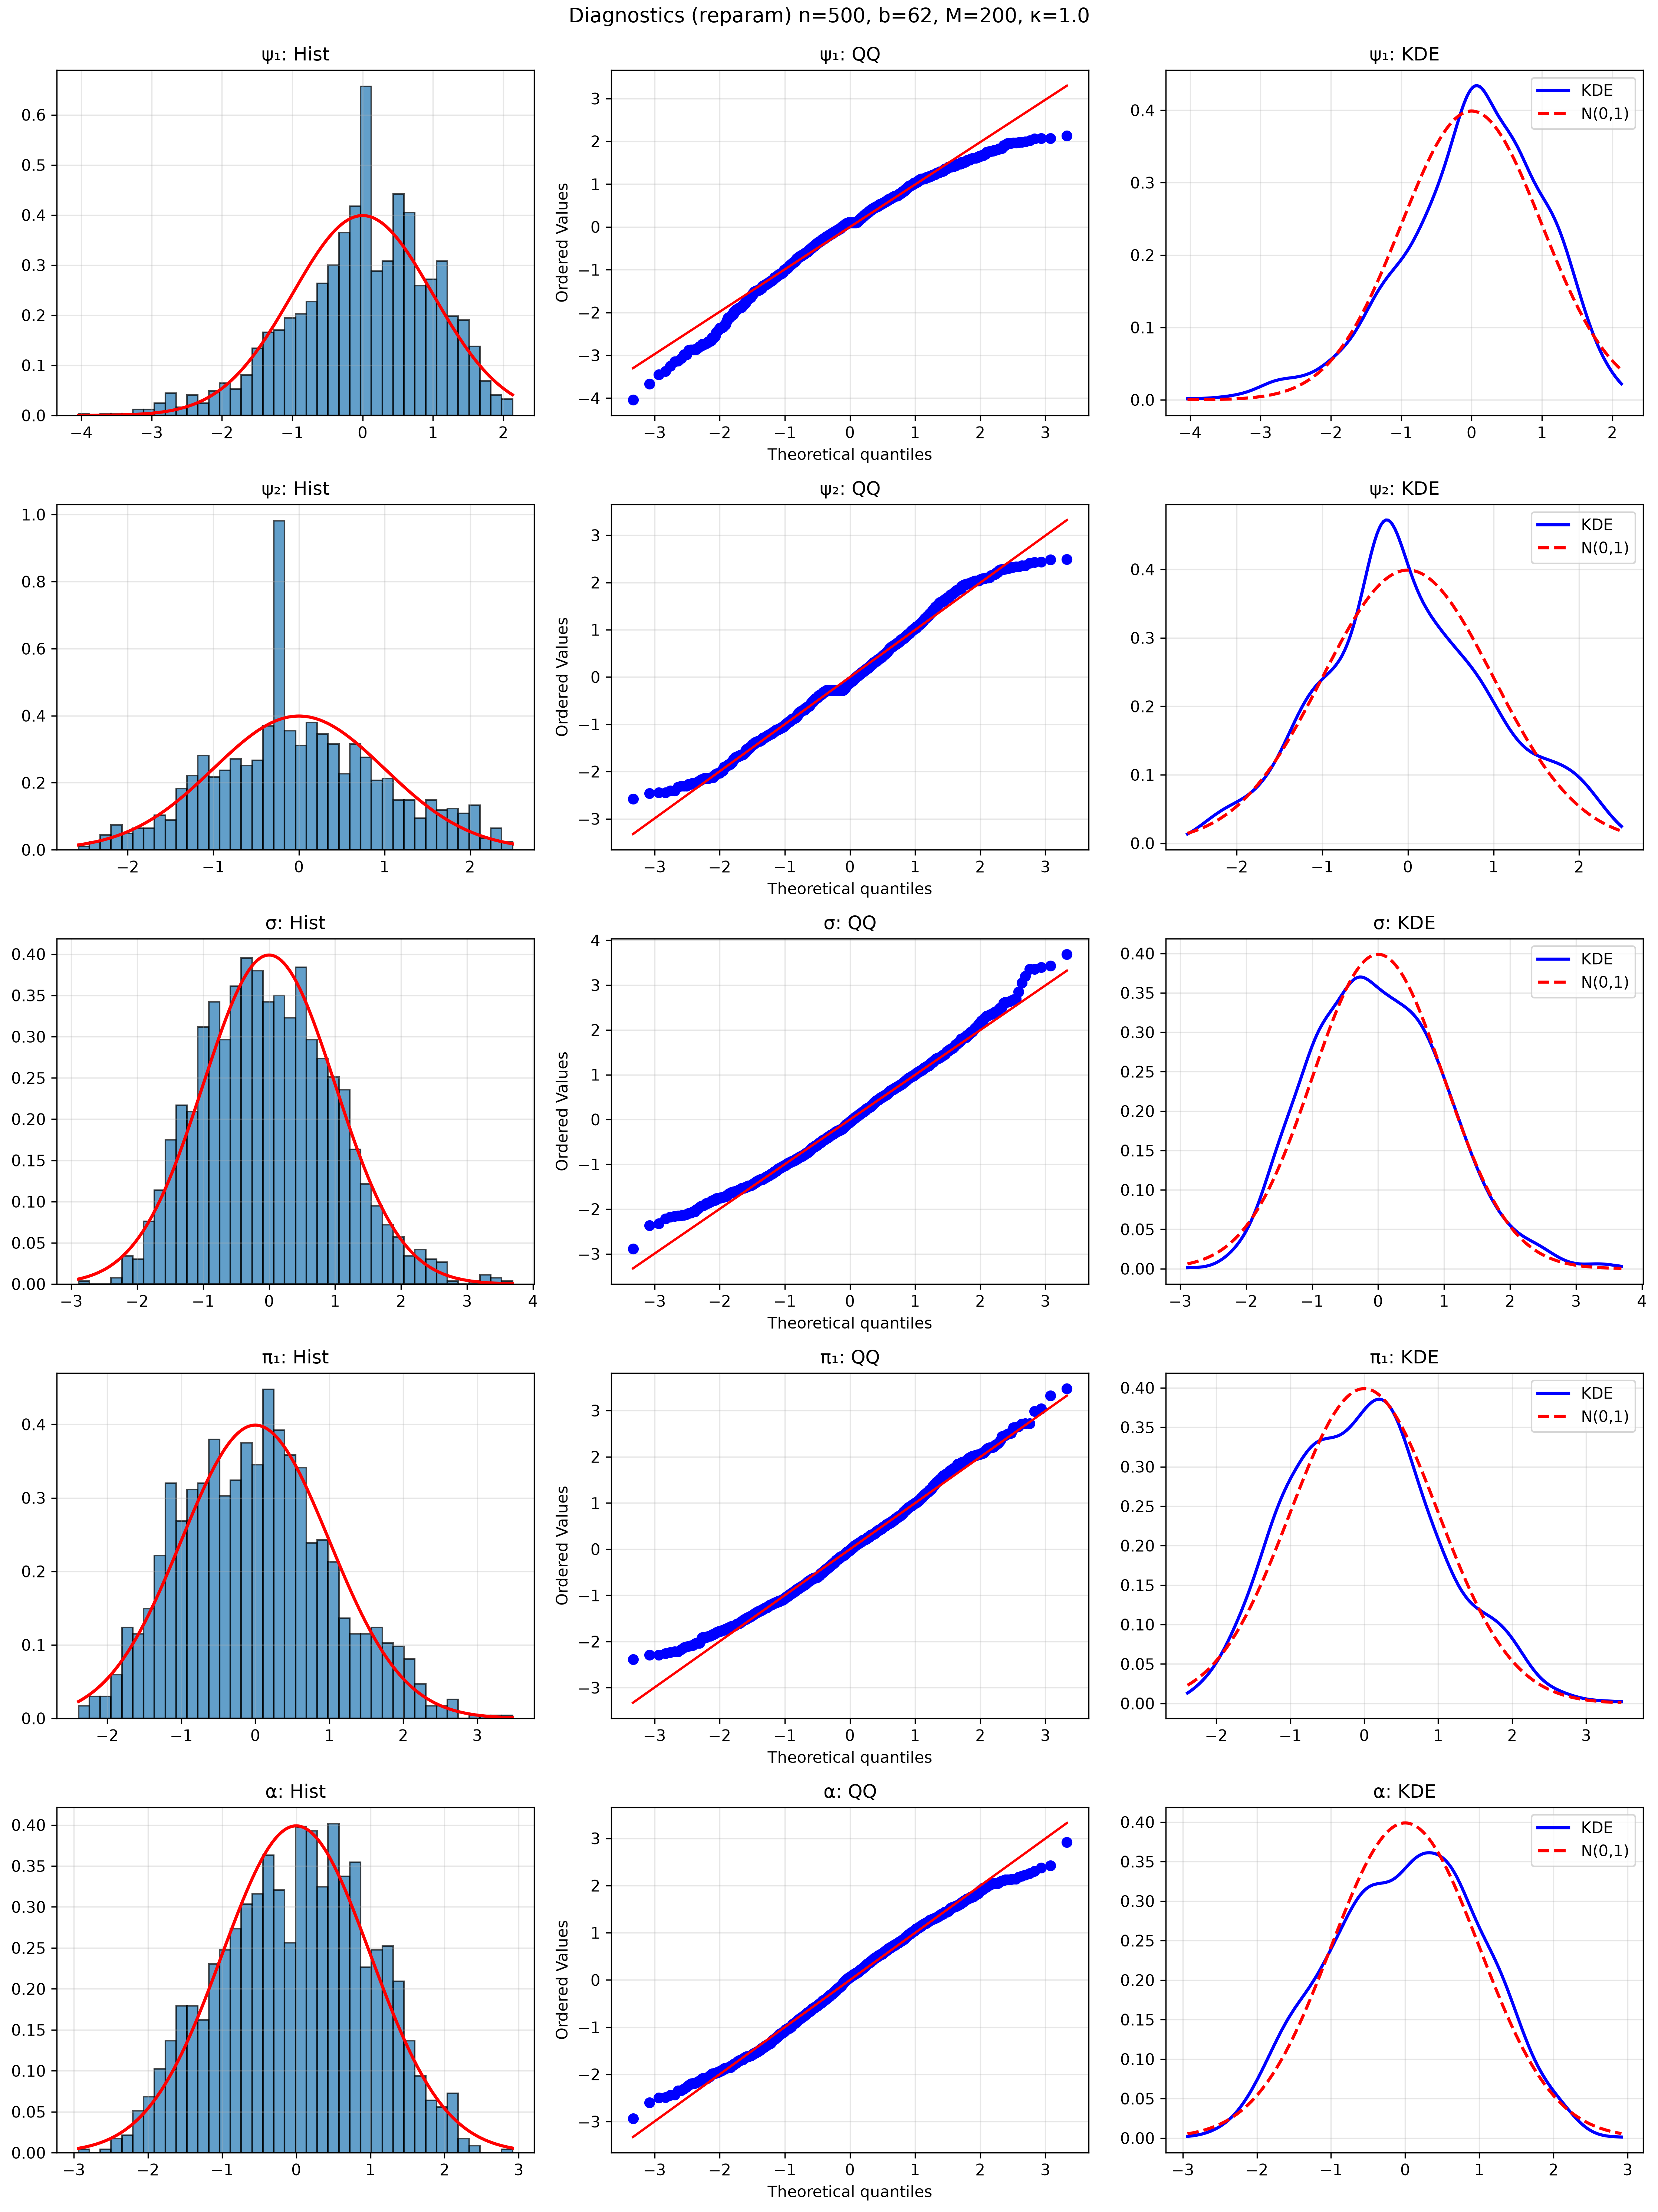
\includegraphics[width=\textwidth]{results_reparam/diagnostics_n500.png}
\caption{Diagnostic plots for scaled subsample deviations (reparameterized) at $n = 500$. For each parameter (rows), we display: (left) histogram with standard normal overlay, (center) Q-Q plot against standard normal quantiles, and (right) kernel density estimate compared to the standard normal density.}
\label{fig:diagnostics_n500}
\end{figure}


\begin{table}[htbp]
\centering
\caption{Subsampling results (reparameterized) for $n = 1{,}000$ ($b = 99$, $N_b = 10$, $M = 200$)}
\label{tab:subsampling_n1000}
\resizebox{\textwidth}{!}{%
\begin{tabular}{lcccccccccccccc}
\toprule
& & & & & & & & & & \multicolumn{2}{c}{Quantile CI} & \multicolumn{2}{c}{Normal CI} \\
\cmidrule(lr){10-11} \cmidrule(lr){12-13}
Parameter & True & Avg Est.\ & Std Est.\ & Dev.\ Mean & Dev.\ Std & Skew & Kurt & SW Rej.\ & JB Rej.\ & qCov90 & qCov95 & nCov90 & nCov95 \\
\midrule
$\psi_1$ & 0.800 & 0.803 & 0.073 & $-0.05$ & 1.552 & $-0.32$ & $0.00$ & 0.190 & 0.000 & 0.605 & 0.650 & 0.785 & 0.810 \\
$\psi_2$ & 0.300 & 0.269 & 0.161 & $0.92$ & 2.849 & $0.15$ & $-0.51$ & 0.320 & 0.000 & 0.455 & 0.460 & 0.620 & 0.690 \\
$\sigma$ & 1.600 & 1.566 & 0.157 & $-0.34$ & 3.828 & $0.27$ & $-0.08$ & 0.075 & 0.000 & 0.685 & 0.720 & 0.760 & 0.815 \\
$\pi_1$ & 0.437 & 0.429 & 0.144 & $-0.87$ & 2.352 & $0.24$ & $-0.10$ & 0.130 & 0.010 & 0.380 & 0.450 & 0.565 & 0.655 \\
$\alpha$ & 1.500 & 1.502 & 0.079 & $0.34$ & 2.347 & $-0.11$ & $-0.51$ & 0.040 & 0.005 & 0.790 & 0.835 & 0.865 & 0.920 \\
\bottomrule
\end{tabular}%
}
\begin{flushleft}
\footnotesize\textit{Notes:} See notes to Table~\ref{tab:subsampling_n500}.
\end{flushleft}
\end{table}


\begin{figure}[htbp]
\centering
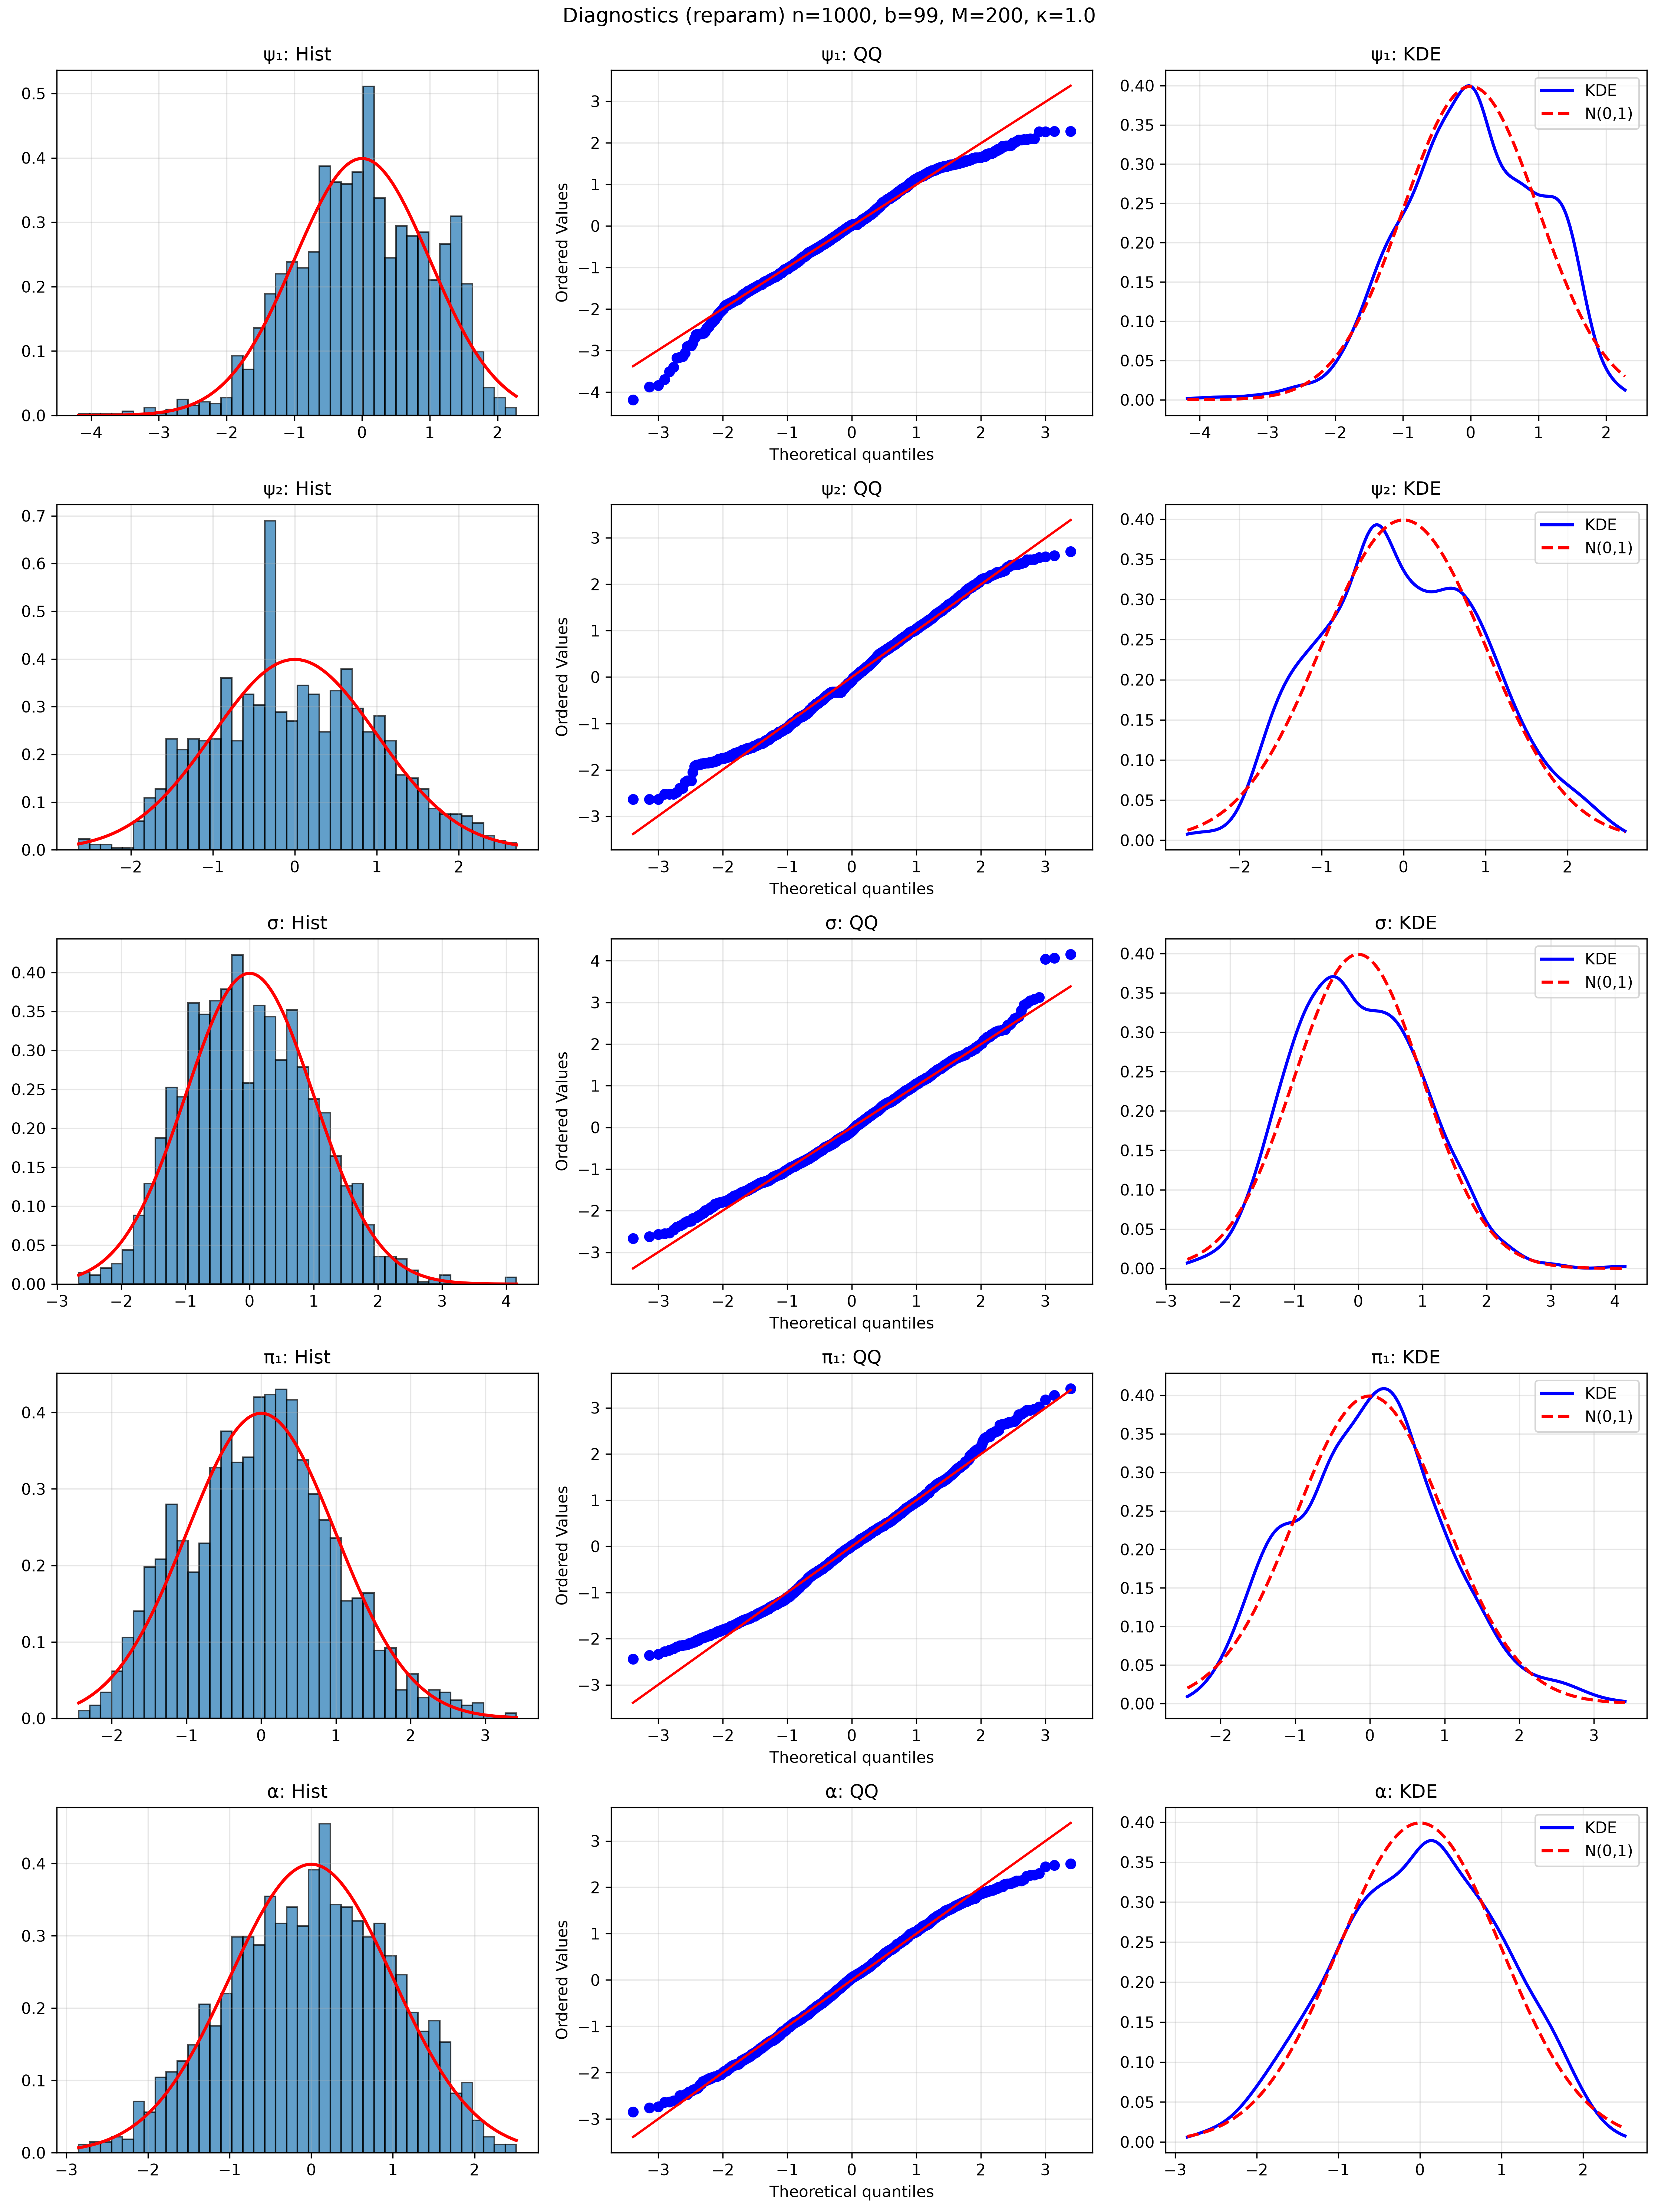
\includegraphics[width=\textwidth]{results_reparam/diagnostics_n1000.png}
\caption{Diagnostic plots for scaled subsample deviations (reparameterized) at $n = 1{,}000$. See caption to Figure~\ref{fig:diagnostics_n500} for details.}
\label{fig:diagnostics_n1000}
\end{figure}


\begin{table}[htbp]
\centering
\caption{Subsampling results (reparameterized) for $n = 10{,}000$ ($b = 464$, $N_b = 21$, $M = 200$)}
\label{tab:subsampling_n10000}
\resizebox{\textwidth}{!}{%
\begin{tabular}{lcccccccccccccc}
\toprule
& & & & & & & & & & \multicolumn{2}{c}{Quantile CI} & \multicolumn{2}{c}{Normal CI} \\
\cmidrule(lr){10-11} \cmidrule(lr){12-13}
Parameter & True & Avg Est.\ & Std Est.\ & Dev.\ Mean & Dev.\ Std & Skew & Kurt & SW Rej.\ & JB Rej.\ & qCov90 & qCov95 & nCov90 & nCov95 \\
\midrule
$\psi_1$ & 0.800 & 0.801 & 0.019 & $0.21$ & 2.186 & $0.22$ & $-0.50$ & 0.240 & 0.005 & 0.865 & 0.900 & 0.920 & 0.970 \\
$\psi_2$ & 0.300 & 0.293 & 0.044 & $0.23$ & 4.403 & $0.13$ & $-0.77$ & 0.290 & 0.000 & 0.780 & 0.795 & 0.890 & 0.945 \\
$\sigma$ & 1.600 & 1.597 & 0.051 & $-1.25$ & 4.718 & $0.11$ & $-0.44$ & 0.065 & 0.005 & 0.830 & 0.865 & 0.845 & 0.920 \\
$\pi_1$ & 0.437 & 0.437 & 0.039 & $-1.05$ & 3.895 & $-0.31$ & $-0.41$ & 0.230 & 0.020 & 0.830 & 0.855 & 0.905 & 0.945 \\
$\alpha$ & 1.500 & 1.501 & 0.026 & $0.15$ & 2.593 & $-0.08$ & $-0.10$ & 0.055 & 0.030 & 0.895 & 0.955 & 0.900 & 0.940 \\
\bottomrule
\end{tabular}%
}
\begin{flushleft}
\footnotesize\textit{Notes:} See notes to Table~\ref{tab:subsampling_n500}.
\end{flushleft}
\end{table}


\begin{figure}[htbp]
\centering
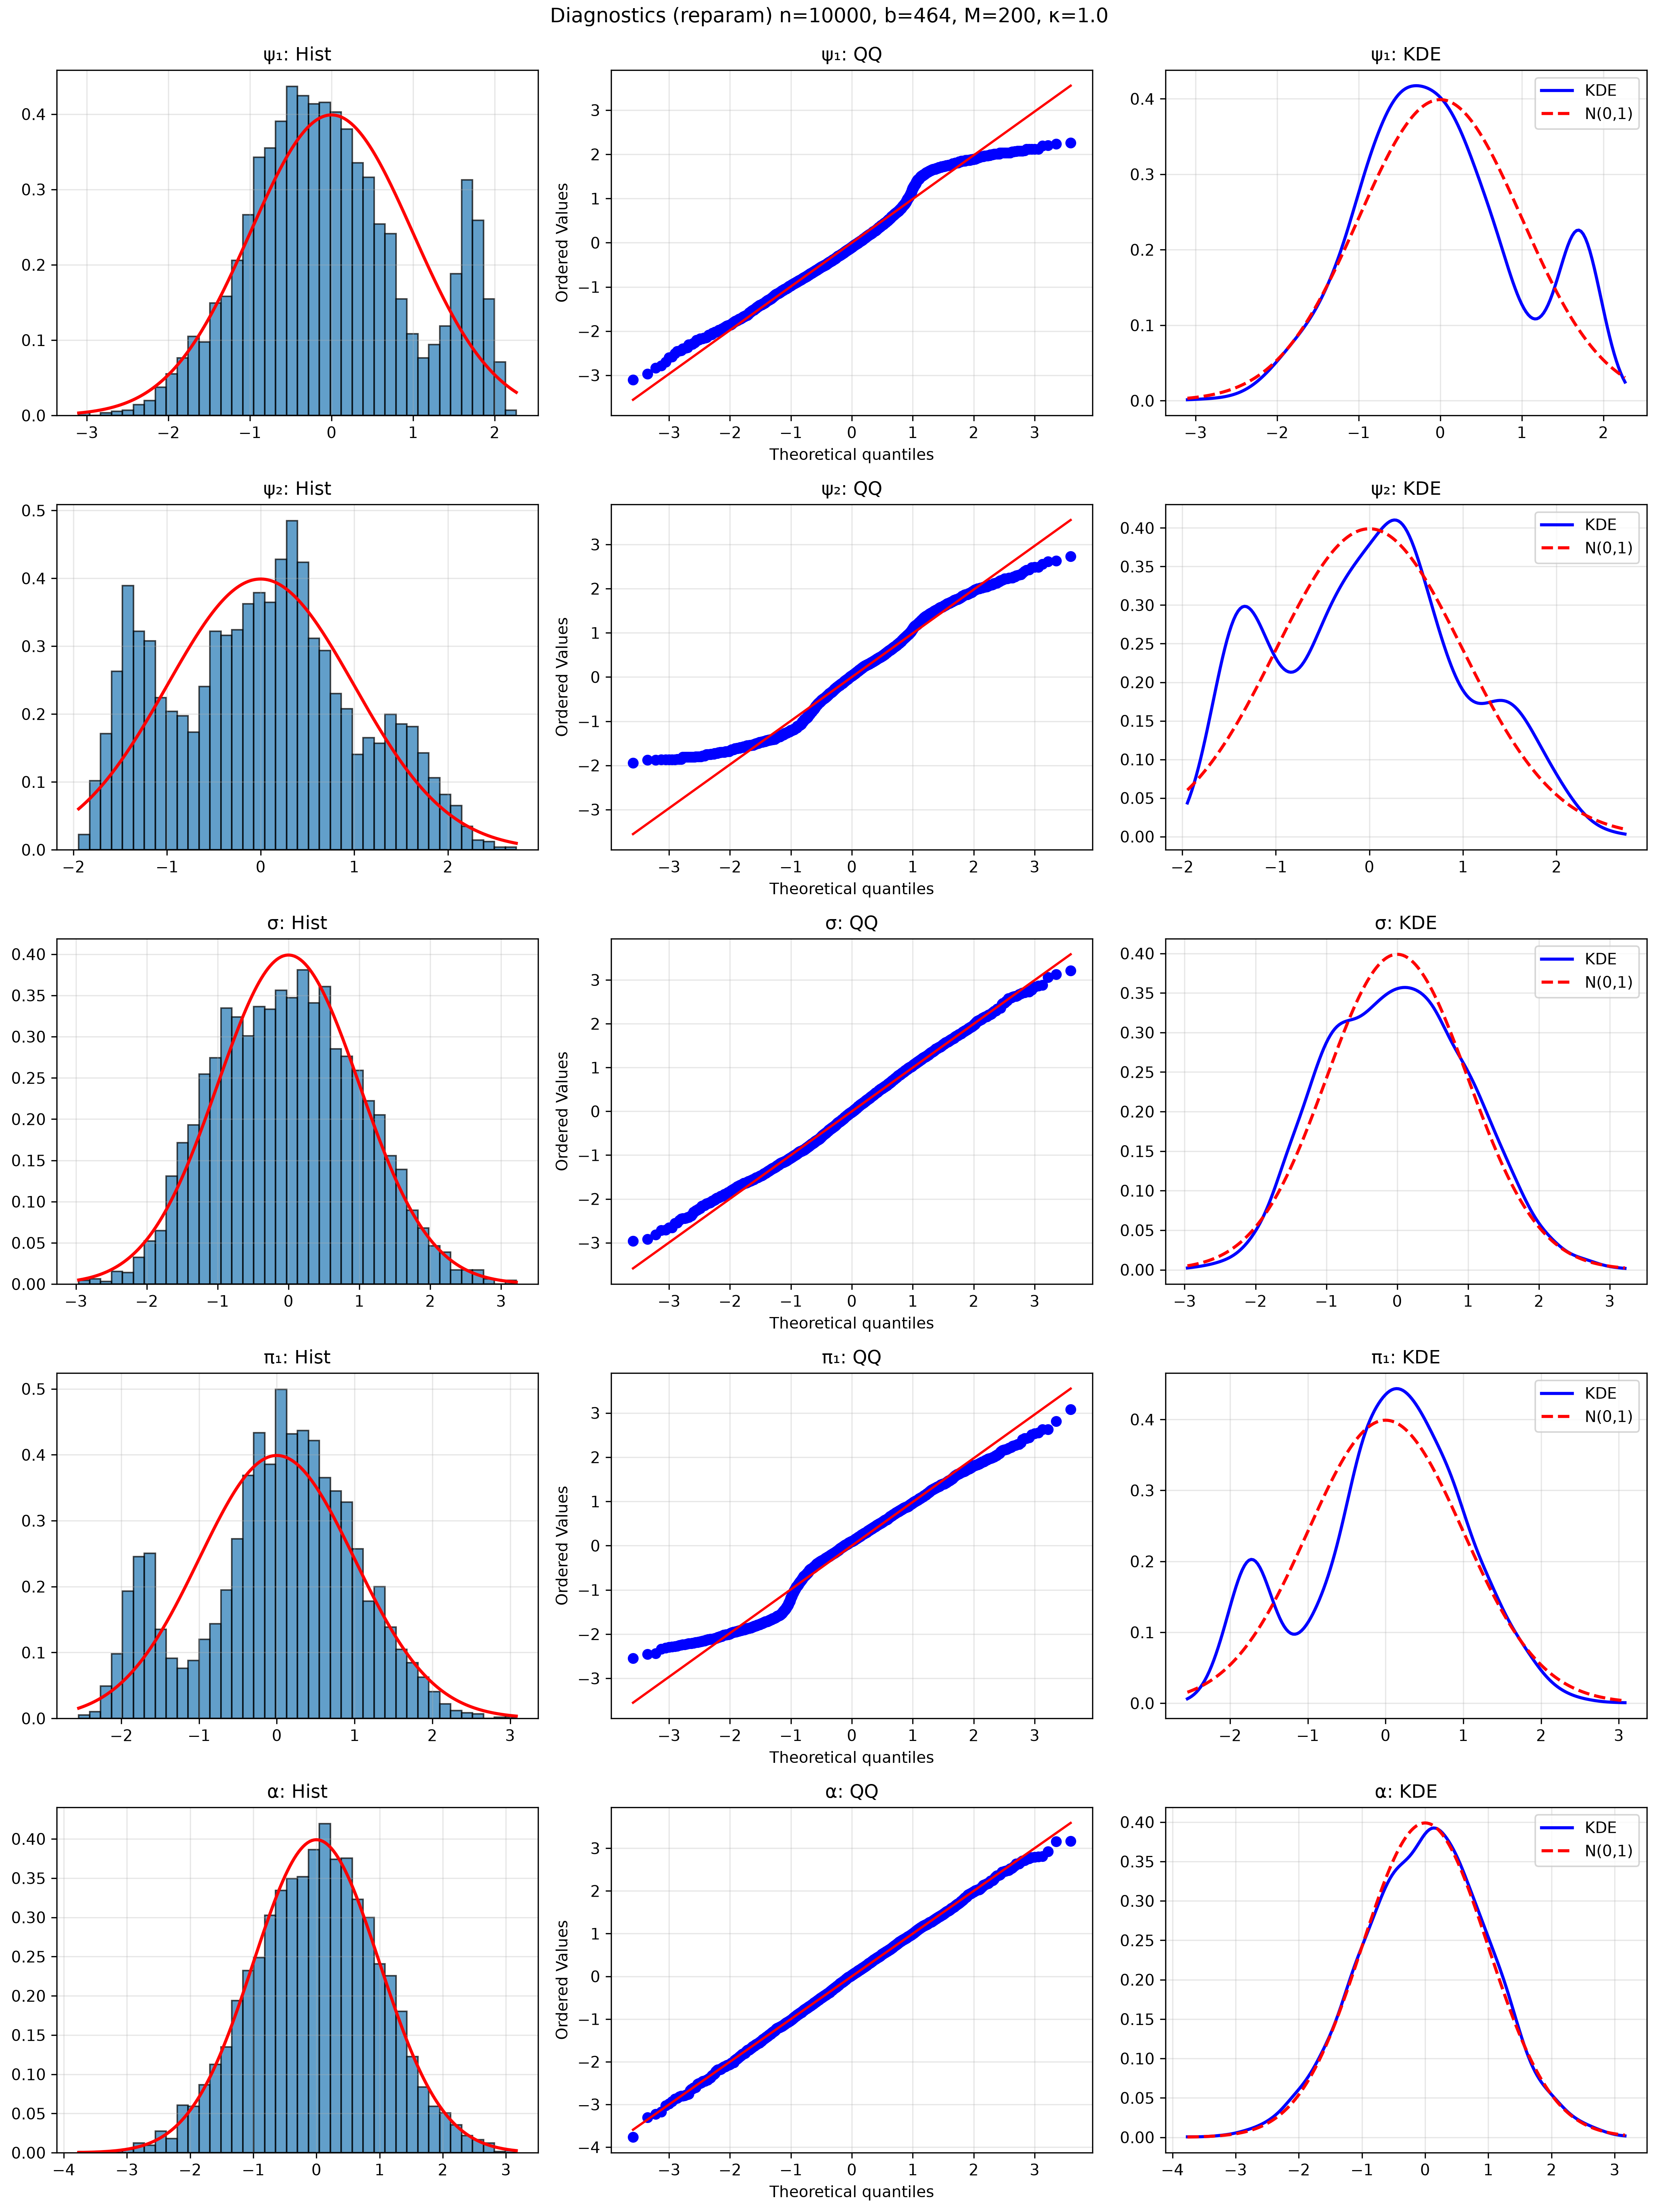
\includegraphics[width=\textwidth]{results_reparam/diagnostics_n10000.png}
\caption{Diagnostic plots for scaled subsample deviations (reparameterized) at $n = 10{,}000$. See caption to Figure~\ref{fig:diagnostics_n500} for details.}
\label{fig:diagnostics_n10000}
\end{figure}


\begin{table}[htbp]
\centering
\caption{Subsampling results (reparameterized) for $n = 100{,}000$ ($b = 2{,}154$, $N_b = 46$, $M = 200$)}
\label{tab:subsampling_n100000}
\resizebox{\textwidth}{!}{%
\begin{tabular}{lcccccccccccccc}
\toprule
& & & & & & & & & & \multicolumn{2}{c}{Quantile CI} & \multicolumn{2}{c}{Normal CI} \\
\cmidrule(lr){10-11} \cmidrule(lr){12-13}
Parameter & True & Avg Est.\ & Std Est.\ & Dev.\ Mean & Dev.\ Std & Skew & Kurt & SW Rej.\ & JB Rej.\ & qCov90 & qCov95 & nCov90 & nCov95 \\
\midrule
$\psi_1$ & 0.800 & 0.801 & 0.006 & $0.11$ & 2.380 & $0.94$ & $2.03$ & 0.595 & 0.590 & 0.940 & 0.970 & 0.935 & 0.990 \\
$\psi_2$ & 0.300 & 0.301 & 0.013 & $-0.55$ & 5.146 & $-0.65$ & $0.64$ & 0.625 & 0.330 & 0.925 & 0.950 & 0.955 & 0.980 \\
$\sigma$ & 1.600 & 1.599 & 0.015 & $-0.82$ & 5.115 & $-0.24$ & $0.19$ & 0.085 & 0.095 & 0.925 & 0.960 & 0.935 & 0.965 \\
$\pi_1$ & 0.437 & 0.436 & 0.012 & $-0.13$ & 4.826 & $-0.79$ & $1.96$ & 0.475 & 0.545 & 0.950 & 0.995 & 0.965 & 0.995 \\
$\alpha$ & 1.500 & 1.501 & 0.008 & $0.07$ & 2.692 & $-0.01$ & $0.02$ & 0.050 & 0.025 & 0.905 & 0.940 & 0.890 & 0.950 \\
\bottomrule
\end{tabular}%
}
\begin{flushleft}
\footnotesize\textit{Notes:} See notes to Table~\ref{tab:subsampling_n500}.
\end{flushleft}
\end{table}


\begin{figure}[htbp]
\centering
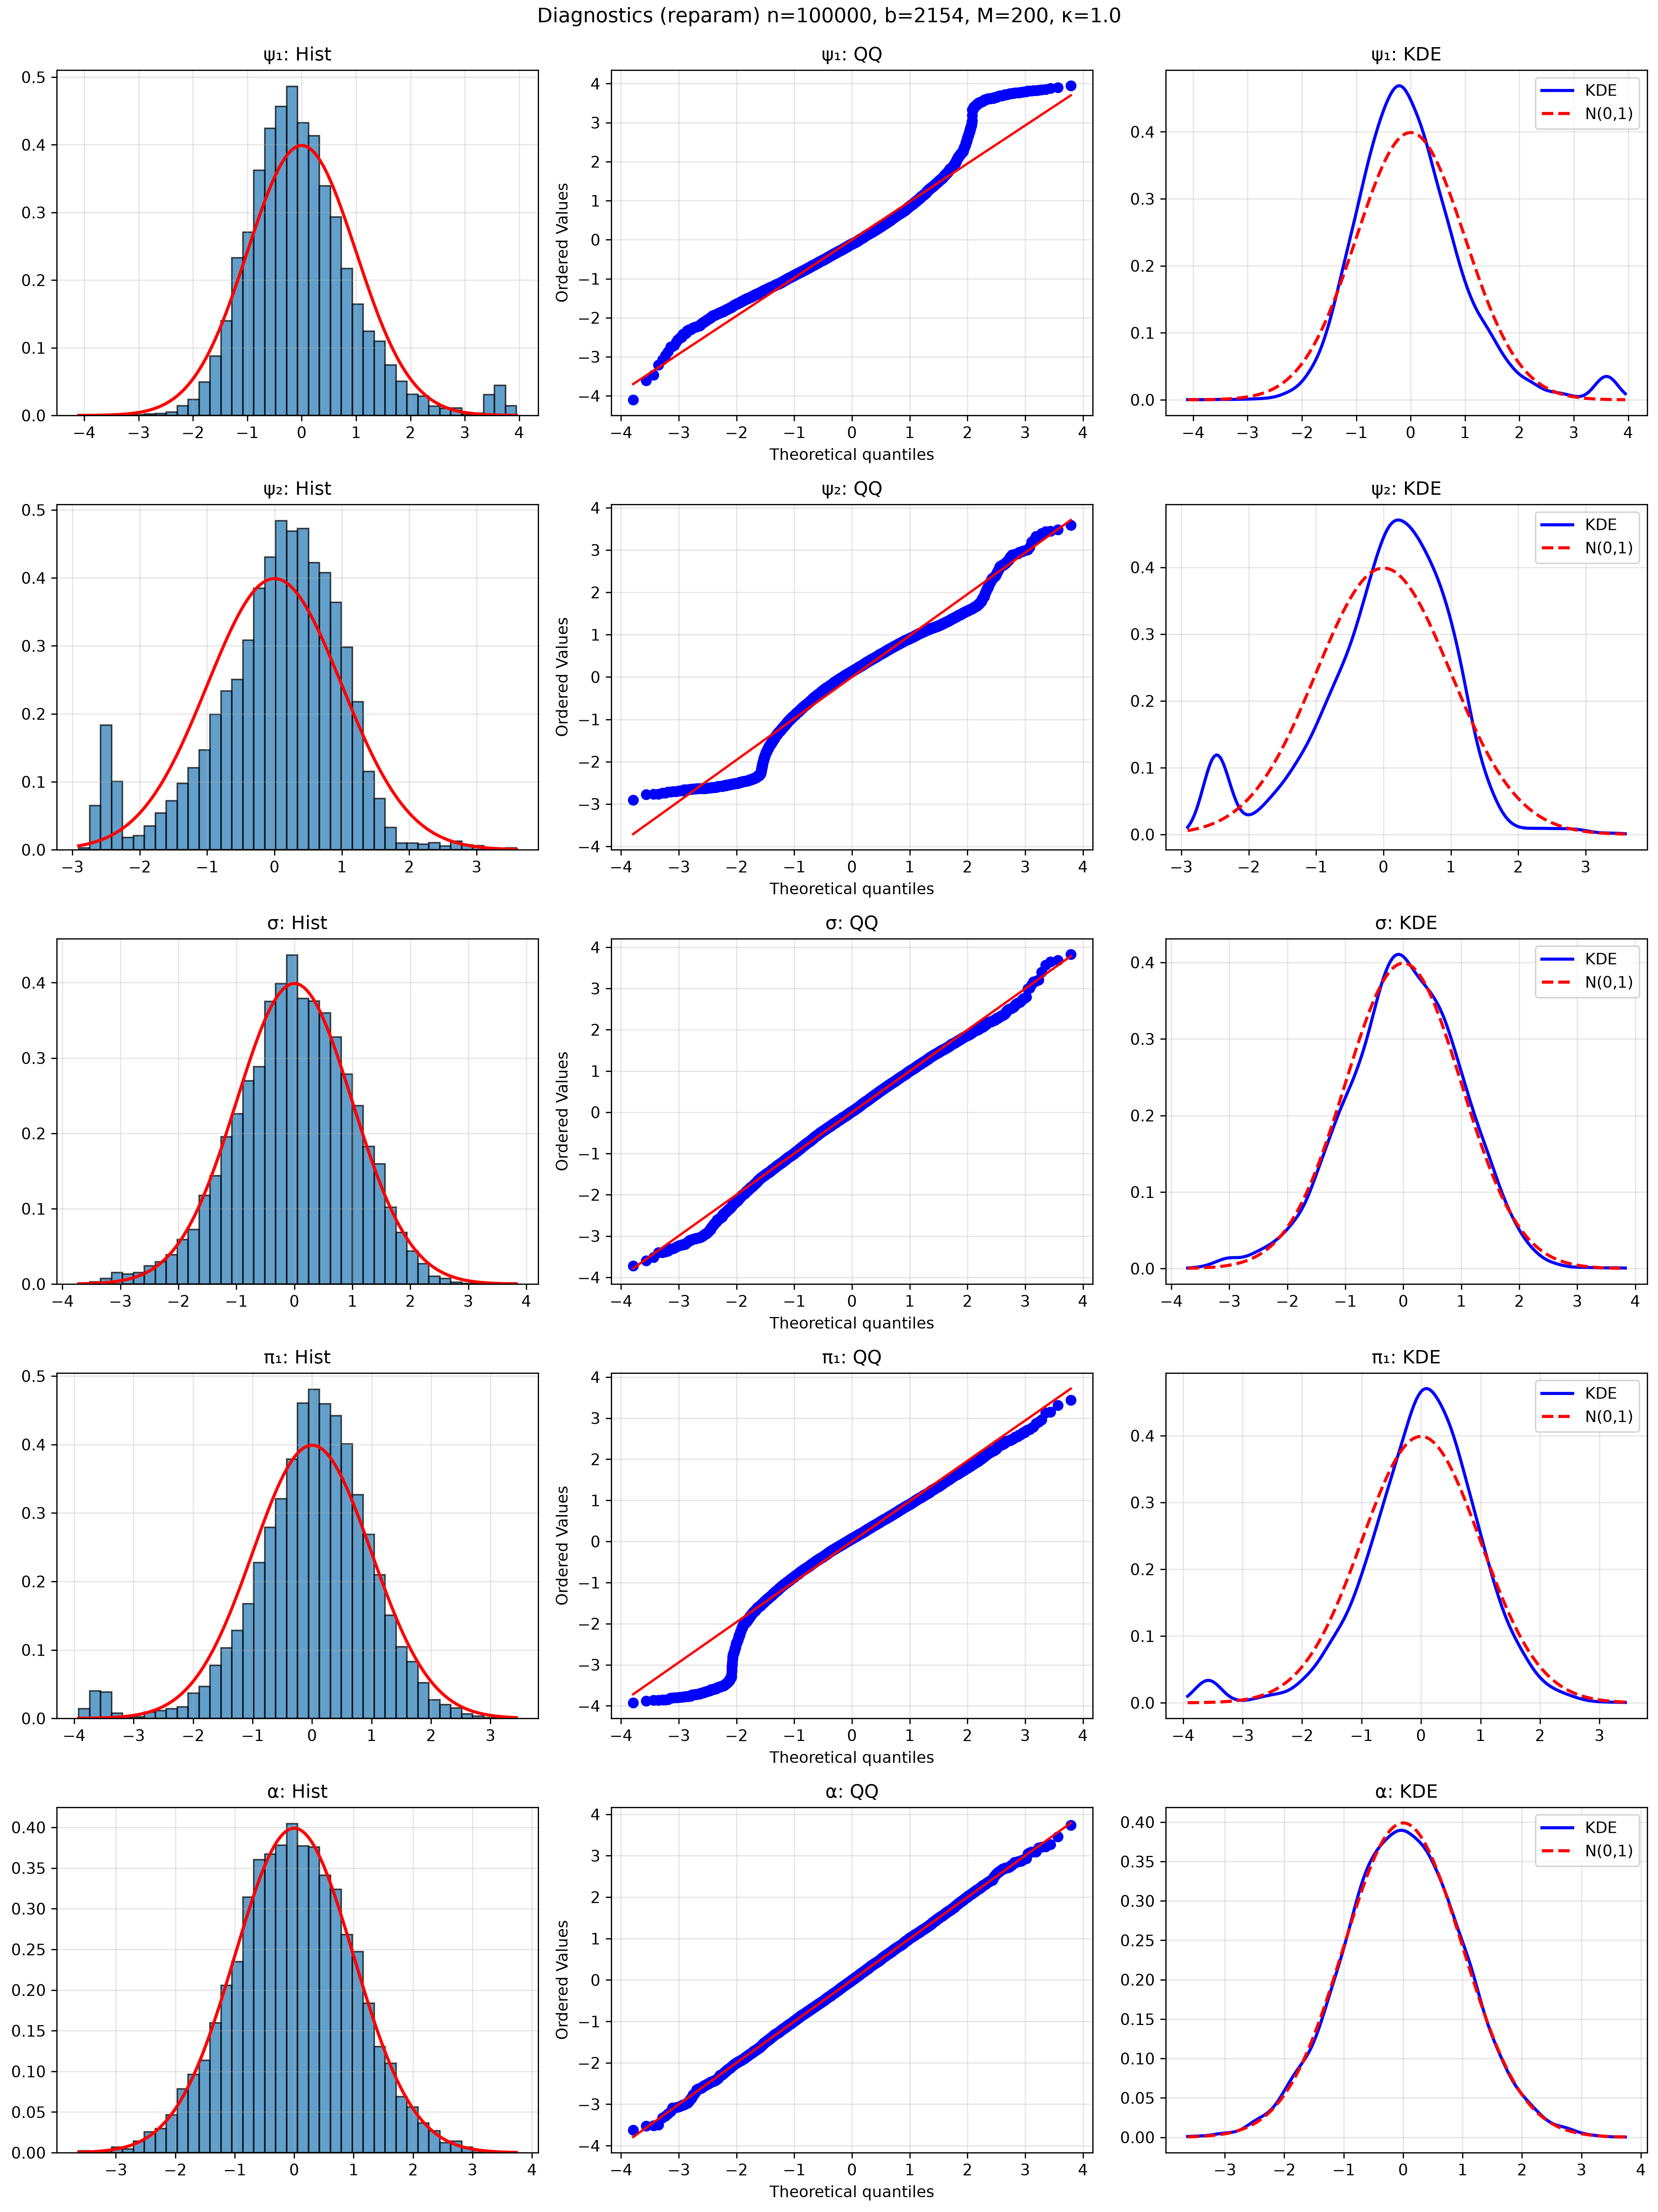
\includegraphics[width=\textwidth]{results_reparam/diagnostics_n100000.png}
\caption{Diagnostic plots for scaled subsample deviations (reparameterized) at $n = 100{,}000$. See caption to Figure~\ref{fig:diagnostics_n500} for details.}
\label{fig:diagnostics_n100000}
\end{figure}


\begin{table}[htbp]
\centering
\caption{Subsampling results (reparameterized) for $n = 500{,}000$ ($b = 6{,}299$, $N_b = 79$, $M = 200$)}
\label{tab:subsampling_n500000}
\resizebox{\textwidth}{!}{%
\begin{tabular}{lcccccccccccccc}
\toprule
& & & & & & & & & & \multicolumn{2}{c}{Quantile CI} & \multicolumn{2}{c}{Normal CI} \\
\cmidrule(lr){10-11} \cmidrule(lr){12-13}
Parameter & True & Avg Est.\ & Std Est.\ & Dev.\ Mean & Dev.\ Std & Skew & Kurt & SW Rej.\ & JB Rej.\ & qCov90 & qCov95 & nCov90 & nCov95 \\
\midrule
$\psi_1$ & 0.800 & 0.800 & 0.003 & $0.03$ & 2.099 & $0.49$ & $1.53$ & 0.260 & 0.275 & 0.925 & 0.965 & 0.910 & 0.950 \\
$\psi_2$ & 0.300 & 0.299 & 0.006 & $-0.30$ & 4.779 & $-0.73$ & $1.63$ & 0.460 & 0.420 & 0.940 & 0.965 & 0.955 & 0.980 \\
$\sigma$ & 1.600 & 1.599 & 0.006 & $-0.35$ & 5.045 & $-0.06$ & $0.14$ & 0.090 & 0.065 & 0.940 & 0.960 & 0.930 & 0.955 \\
$\pi_1$ & 0.437 & 0.437 & 0.005 & $0.01$ & 4.251 & $-0.33$ & $1.44$ & 0.170 & 0.195 & 0.925 & 0.970 & 0.930 & 0.965 \\
$\alpha$ & 1.500 & 1.500 & 0.004 & $0.04$ & 2.763 & $0.01$ & $-0.01$ & 0.070 & 0.045 & 0.910 & 0.950 & 0.900 & 0.945 \\
\bottomrule
\end{tabular}%
}
\begin{flushleft}
\footnotesize\textit{Notes:} See notes to Table~\ref{tab:subsampling_n500}.
\end{flushleft}
\end{table}


\begin{figure}[htbp]
\centering
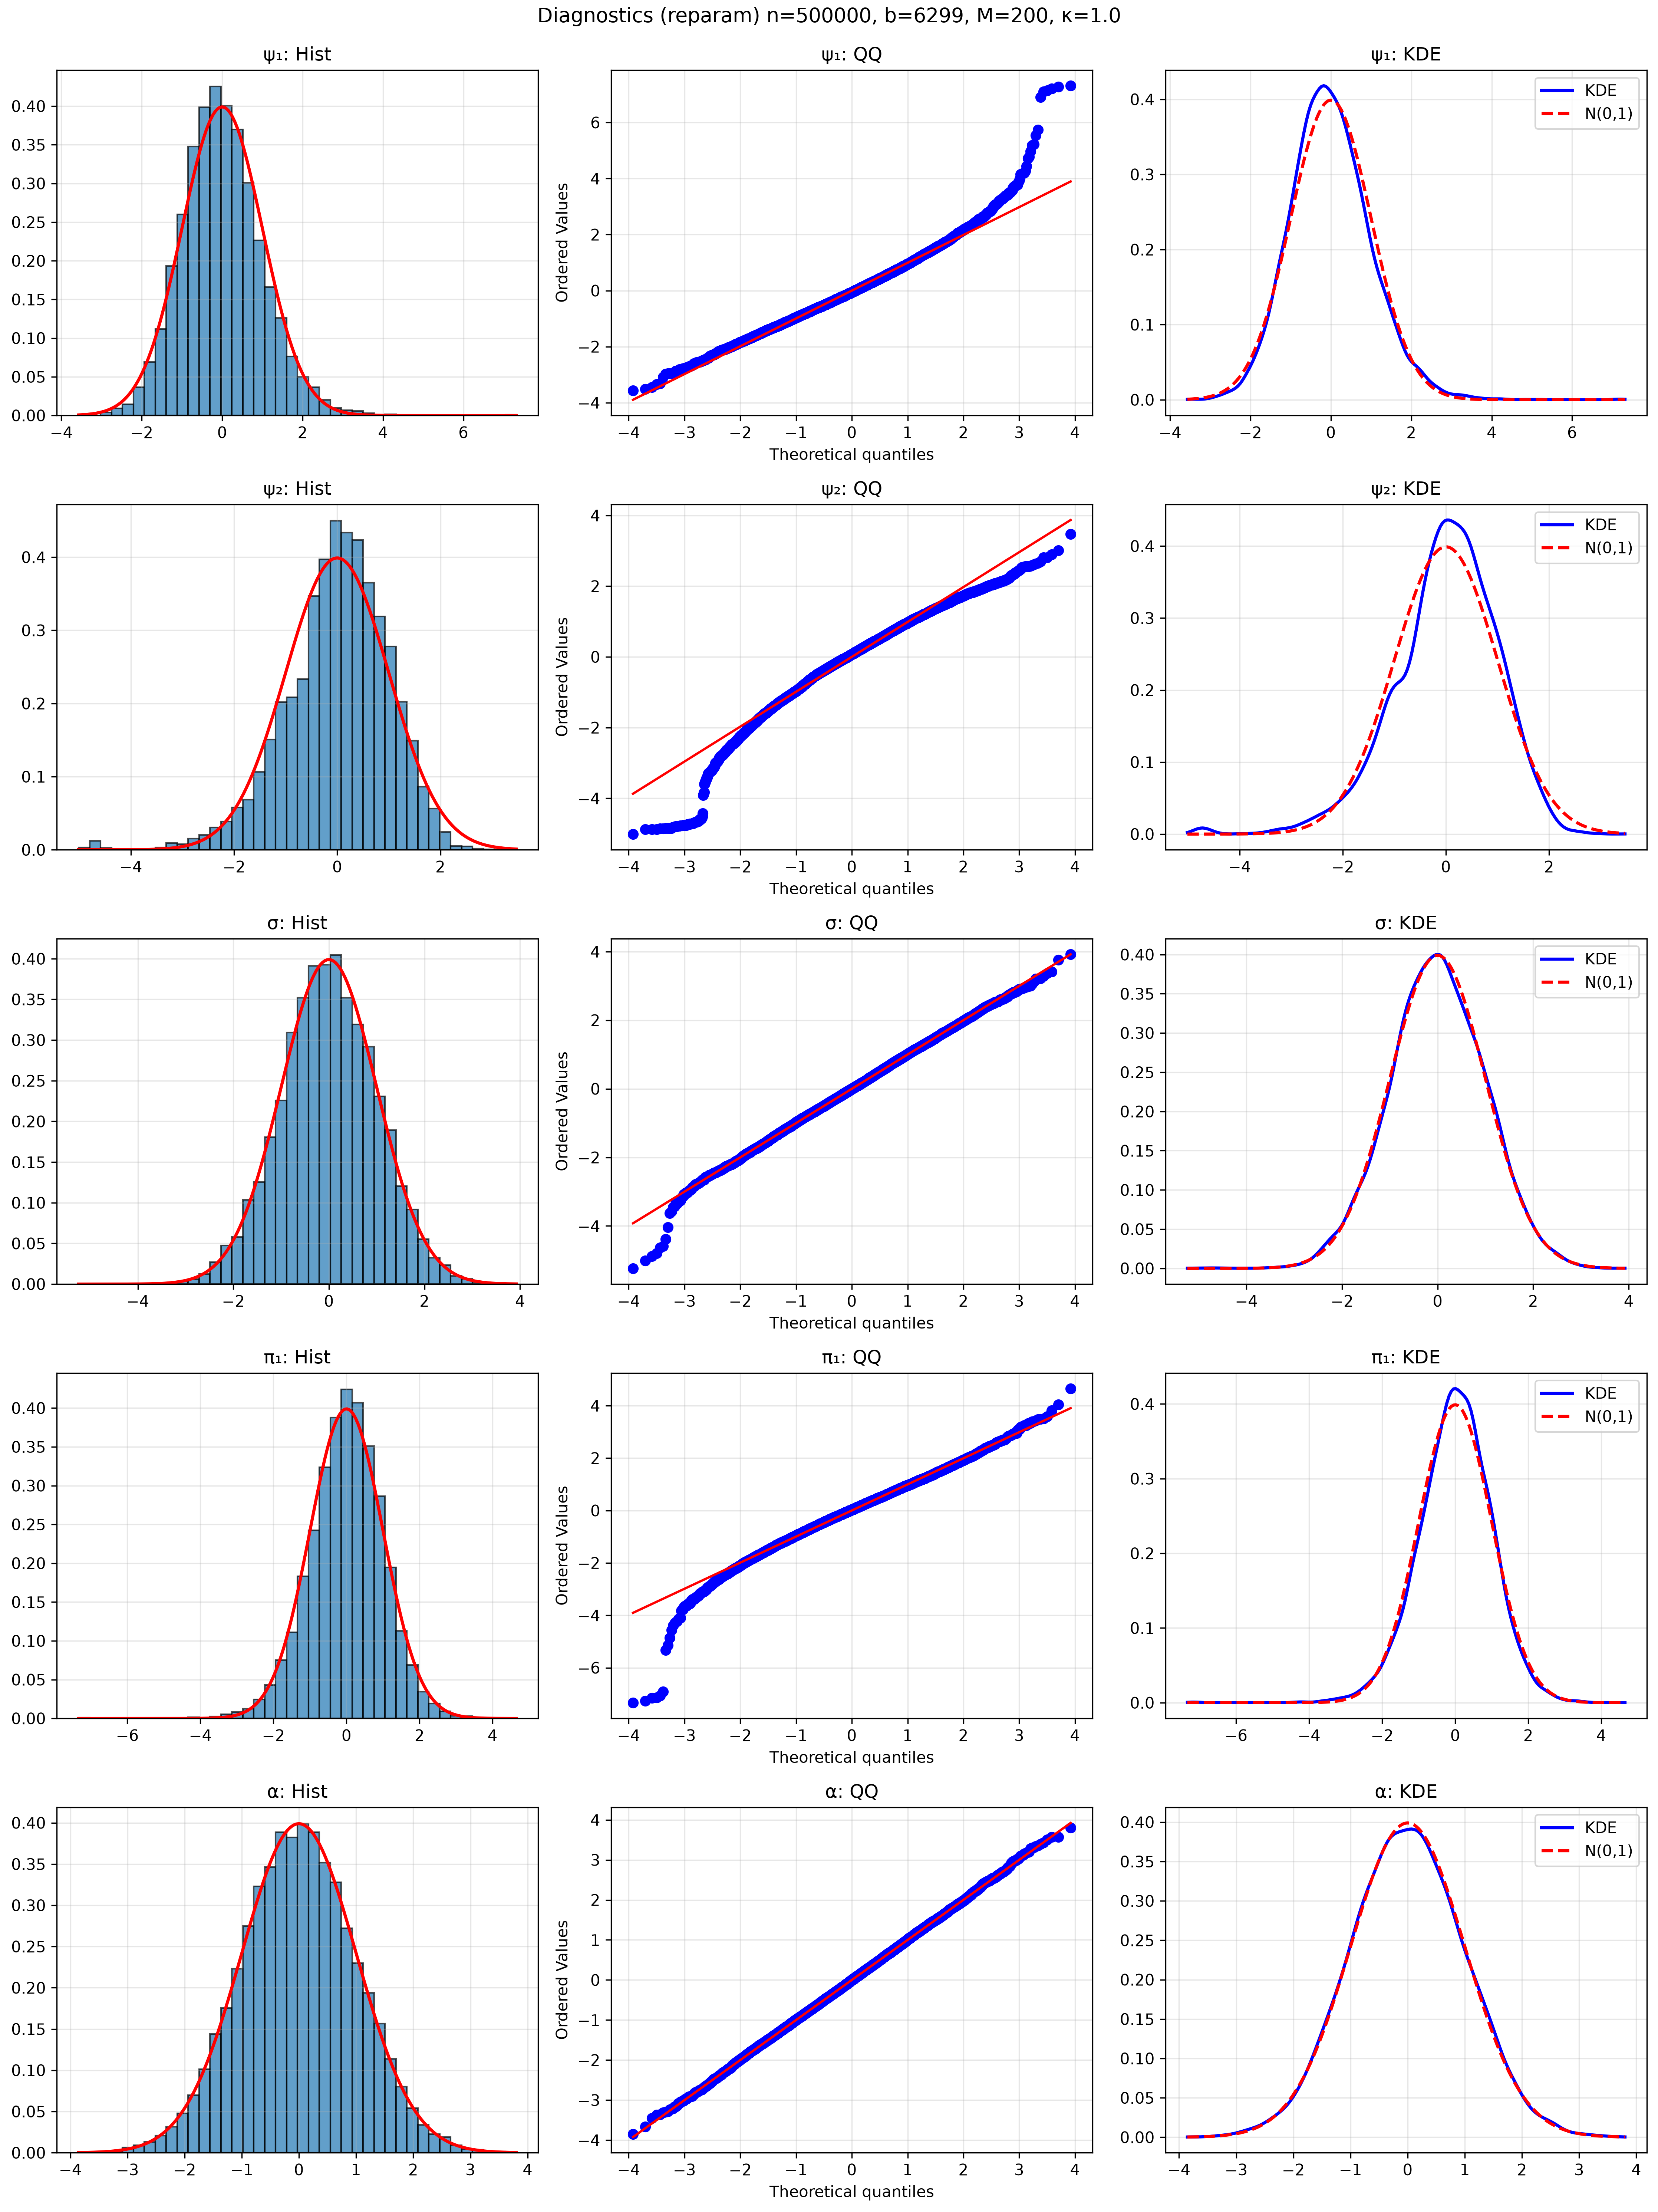
\includegraphics[width=\textwidth]{results_reparam/diagnostics_n500000.png}
\caption{Diagnostic plots for scaled subsample deviations (reparameterized) at $n = 500{,}000$. See caption to Figure~\ref{fig:diagnostics_n500} for details.}
\label{fig:diagnostics_n500000}
\end{figure}
